\documentclass{cslthse-msc}
\usepackage[utf8]{inputenc}
\usepackage[english]{babel}
\usepackage{amsmath}
\usepackage{amsfonts}
\usepackage{amssymb}
\usepackage{amsthm}
%\usepackage{makeidx}
\usepackage{graphicx}
\usepackage[titletoc, header, page]{appendix}

\usepackage{hyperref}
\usepackage{pdfpages}

\usepackage{enumitem}
\usepackage{subfig}
\usepackage{float}
\usepackage{listings}
%% listings-modelica.cfg
%% Copyright 2014 Martin Sjoelund, Dietmar Winkler
%
% This work may be distributed and/or modified under the
% conditions of the LaTeX Project Public License, either version 1.3
% of this license or (at your option) any later version.
% The latest version of this license is in
%   http://www.latex-project.org/lppl.txt
% and version 1.3 or later is part of all distributions of LaTeX
% version 2005/12/01 or later.
%
% This work has the LPPL maintenance status `maintained'.
%
% The Current Maintainer of this work is Dietmar Winkler
%
% Code repository https://github.com/modelica-tools/listings-modelica
%
% This work consists of the file listings-modelica.cfg

\lstdefinelanguage{modelica}
{
  morekeywords=[1]{
    algorithm,and,annotation,as,assert,block,break,case,class,connect,connector,
    constant,constrainedby,der,discrete,each,else,elseif,elsewhen,encapsulated,
    end,enumeration,equality,equation,expandable,extends,external,failure,final,
    flow,for,function,guard,if,import,in,initial,inner,input,List,local,loop,
    match,matchcontinue,model,not,operator,Option,or,outer,output,package,parameter,
    partial,protected,public,record,redeclare,replaceable,return,stream,
    subtypeof,then,Tuple,type,uniontype,when,while},
  morekeywords=[2]{true, false},
  % Do not make true,false keywords because fn(true,x, false ) shows up as fn(true,x, *false*)
  sensitive=true,
  comment=[l]//,
  morecomment=[s]{/*}{*/},
  alsodigit={.,-},
  morestring=[b]',
  morestring=[b]",
}[keywords,comments,strings]

\definecolor{keywordcolor1}{rgb}{0,0,.4}
\definecolor{keywordcolor2}{rgb}{.90,0,0}
\definecolor{stringcolor}{rgb}{0.133,0.545,0.133}
% \definecolor{listingbgcolor}{rgb}{0.95,0.95,0.95}

\lstset{
  breaklines=true,
  language=modelica,
  basicstyle=\ttfamily,
  keywordstyle=[1]\color{keywordcolor1}\bfseries,
  keywordstyle=[2]\color{keywordcolor2},
  stringstyle=\color{stringcolor},
%  backgroundcolor=\color{listingbgcolor},
  framexleftmargin=5pt,
  xleftmargin=5pt,
  xrightmargin=5pt,
  showstringspaces=false
}

\newcommand{\code}[1]{\lstinline|#1|}
\newcommand{\modelica}[1]{\lstinline[language=modelica]|#1|}


%\geometry{showframe}

\author{
	Erik Hedblom \\
	{\normalsize \href{mailto:hedblom.e@gmail.com}{\texttt{hedblom.e@gmail.com}}}
	\and
	Kasper Rundquist \\
	{\normalsize \href{mailto:kasper.rundquist@gmail.com}{\texttt{kasper.rundquist@gmail.com}}}
}

\title{Safe regression test selection using static analysis}
%\subtitle{A {\LaTeX} class}
\company{Modelon AB}
\supervisors{Johan Ylikiiskilä, \href{mailto:johan.ylikiiskila@modelon.com}{\texttt{johan.ylikiiskila@modelon.com}}}{Jonatan Kämpe, \href{mailto:jonathan.kampe@modelon.com}{\texttt{jonathan.kampe@modelon.com}}}{Niklas Fors, \href{mailto:niklas.fors@cs.lth.se}{\texttt{niklas.fors@cs.lth.se}}}%\supervisor{Niklas Fors, \href{mailto:niklas.fors@cs.lth.se}{\texttt{niklas.fors@cs.lth.se}}}
\examiner{Görel Hedin, \href{mailto:gorel.hedin@cs.lth.se}{\texttt{gorel.hedin@cs.lth.se}}}

\date{\today}
%\date{January 16, 2015}

\acknowledgements{
If you want to thank people, do it here, on a separate right-hand page. Both the U.S. \textit{acknowledgments} and the British \textit{acknowledgements} spellings are acceptable.
}

\theabstract{
This document describes the Master's Thesis format for the theses carried out at 
the Department of Computer Science, Lund University. 

Your abstract should capture, in English, the whole thesis with focus on the problem and solution in 150 words. It should be placed on a separate right-hand page, with an additional \textit{1cm} margin on both left and right. Avoid acronyms, footnotes, and references in the abstract if possible.

Leave a \textit{2cm} vertical space after the abstract and provide a few keywords relevant for your report. Use five to six words, of which at most two should be from the title.
}

\keywords{Regression Test Selection, Modelica}

\divisionoflabor{
}

%% Only used to display font sizes
\makeatletter
\newcommand\thefontsize[1]{{#1 \f@size pt\par}}
\makeatother
%%%%%%%%%%


\begin{document}
\makefrontmatter
\chapter[Introduction]{Introduction}

\section{Motivation / Background}
During software development, when a change is integrated into a project all previous testing have to be rerun. Test suites usually accumulates over time and regression testing can therefore be very time consuming. Depending on the change some or most of the test may be unrelated to the change and by excluding unrelated tests significant time savings could be achieved. ~\cite{DUMMY}


Det är viktig att testa mjukvara under utvecklingen för säkerställa att mjukvaran fungerar korrekt. När mjukvaran uppdateras måste testfall som redan testats utföras igen för att kontrollera att allt som fungerade innan uppdatering fortfarande fungerar efter. Det kan vara väldigt tidskrävande att köra samtliga test. Det finns därför mycket tid att spara om det går att utesluta test som garanterat inte har påverkas. För språket Modelica finns det inget verktyg för detta och det är därför intressant att utveckla ett.

\section{Problem Description / Aim / Goal}

The aim of this project is too reduce testing times for Modelica projects without loss of quality. This will be done by developing and implementing a method to exclude tests in a test suite unaffected by a specific change. Regression testing can then be performed with a reduced test suite without compromising quality. 

\chapter[Background]{Background}
\section{Regression Testing}
Regression tests are used to make sure that regression dose not occur. Software regression is when something that did work before do not work as expected due to a change.
\section{Test Selection}
\begin{itemize}
	\item What is test selection?
	\item Different approaches
A safe Regression Test Selection (RTS) method will select all tests that produce a new result after a specific change. A safe RTS method is equivalent to running all tests. For a RTS method to be useful the RTS algorithm should run in less time than it takes to run the excluded tests.
\end{itemize}

\section{Modelica}
\begin{itemize}
	\item What is Modelica?
Modelica is an object-oriented language and is used for physical models and simulation. 

The output of a Modelica compilation process is code to be compiled, in our case C-code.~\cite{aakesson2008development}

\subsection{Classes}
Basically everything in Modelica is classes. Built in types such as Integer are Modelica classes. Packages, models and functions are classes.

Modelica allows short definitions of classes. The definition of a class to the left in figure \ref{fig:classDefinition}, is equivalent to the definition to the right.

\begin{figure}[H]
    \centering
    \subfloat{{\lstinputlisting[language=modelica]{modelica/packageDecl.mo}}}
    \qquad
    \subfloat{{\lstinputlisting[language=modelica]{modelica/shortPackageDecl.mo}}}
    \caption{Class definition}
    \label{fig:classDefinition}
\end{figure}

\subsection{Name lookup}
In order to find a match for a name, Modelica starts by looking at the first name in a qualified name. Take for example the fully qualified name Modelica.Fluid.Pipes.StaticPipe. In this example Modelica is the first name in the qualified name.

To find a match for the name Modelica first checks if it's a built in type. If it's a built in type Modelica has found a match for the name.

If it's not a built in type Modelica looks in the class where the name is used, including inherited definitions, for a nested definition of the name. 

If there is no nested definition of the name, Modelica looks in the imports in the class where the name is used, inherited imports are not included, to find a match for the name.

If a match for the name is not found in the imports, Modelica looks for a nested definition in the parent package, including inherited definitions.

If the definition of the name not is found in the parent package, Modelica looks for a imported definition, not including inherited imports, in the parent package.

If a match for the name still not is found, Modelica continues by using the same method and looking in the parent packages parent package and so on until: the parent package has the encapsulated qualifier or a package doesn't have a parent package. In the first case the search for the name terminates and in the second case Modelica searches for a match in root level packages.

This search is done in the same way for the first name in a qualified name and an unqualified name. An unqualified name doesn't contain a dot, an unqualified name consists of only one name. StaticPipe is an example of an unqualified name.

If a name is a part of a qualified name and isn't the first name in the qualified name, it must be a nested definition within the definition of the previous name in the qualified name. In the example Modelica.Fluid.Pipes.StaticPipe, Fluid must be a nested definition within Modelica.\cite{modelicamodelica, tillermodelica}

\subsection{Access}

\subsection{Redeclear}
	\item How can we perform test selection for Modelica?
	\item SourceTree, InstanceTree, FlatTree
\end{itemize}

\section{JastAdd}
JastAdd is a system based on reference attribute grammars, for extensible implementation of compilers. An Abstract Syntax Tree (AST) is used to represent a program. Attribute Grammars is amethod for declerativly defining computations on an AST. A node in an AST can have a synthezied attribute or an inherited attribute. An attribue is defined by an equation. A synthezied attribyte is defined in the node, an inherired attribute is defined in an ancestor node. A JastAdd specification is used to create an object-oriented framework.~\cite{aakesson2008development}

Collection attributes are defined by partial definitions in a number of arbitrary nodes. A node that have a partial definition of a collection attribute contributes to the value of the collection attribute. A collection attribute is usually a set where the empty set is the initial value of the collection attribute. The contributors, the nodes that contributes to the collection attribute, can for example contribute by adding elements to the set.~\cite{magnusson2007extending}

\chapter[Implementation]{Implementation}

\section{Dependency analysis}
The Dependency analysis should produce a directed graph on dot format. Dot is a plain text representation of a graph, that can be visualized.
\setlist{nolistsep}
\begin{enumerate}[]
\item A class depends on its parent class if it has one.

\item A class depends on all accesses in its immediate subtree.
\begin{enumerate}[]
\item A class depends on the accessed class and all its subclasses.
\item A class depends on all classes in the path to the accessed class.
\end{enumerate}
\end{enumerate}
An immediate subtree is a tree with a single ClassDecl, the ClassDecl is allways the root.
A immediate subtree is created by taking the AST subtree at a ClassDecl node and removing all subtrees with a ClassDecl, ElementRedeclare, child of Access or CompnentModification as root. So that the new tree only contains one ClassDecl, the root.

In figure \ref{fig:extends}, class C is the accessed class in the immediate subtree of class A. Class B is in the path to the accessed class. Class E is an subclass to class C.
Example:
\begin{figure}[H]
    \centering
    \subfloat{{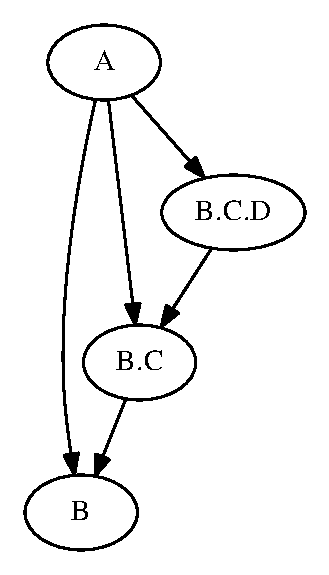
\includegraphics[]{EPS-graphs/extends.eps}}}
    \qquad
    \subfloat{{\lstinputlisting[language=modelica]{modelica/extends.mo}}}
    \caption{Extends Graph}
    \label{fig:extends}
\end{figure}
Dependency rules
\begin{figure}[H]
    \centering
    \subfloat{{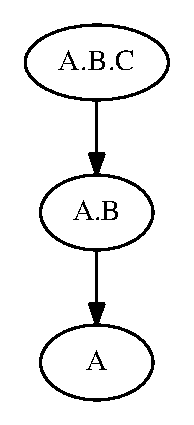
\includegraphics[]{EPS-graphs/ParentExample.eps}}}
    \qquad
    \subfloat{{\lstinputlisting[language=modelica]{modelica/parentExample.mo}}}
    \caption{Parent graph}
    \label{fig:parentGraph}
\end{figure}

There is a constant k defined in package A. If we define a constant k in model B, the k accessed in C will be k defined in model B. Therefore we need a dependency from C to B.

If the constant k in package A is changed it will affect model C. Therefore we need a dependency from C to A. With rule number 1 we get dependencies from C to B and from B to A. So we have an indirect dependency from C to A, figure \ref{fig:parentGraph}.

\begin{figure}[H]
    \centering
    \subfloat{{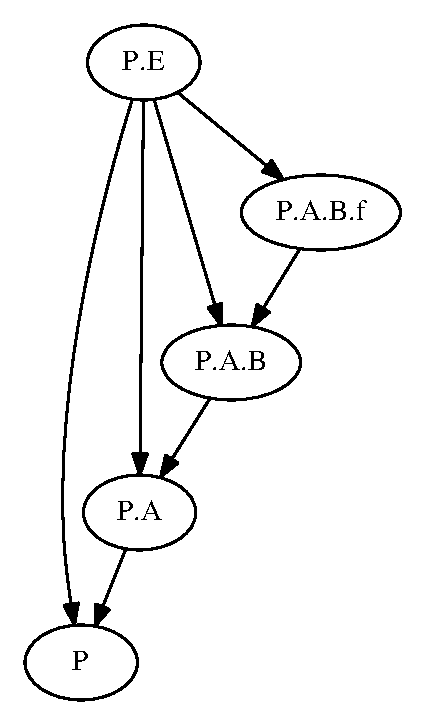
\includegraphics[]{EPS-graphs/GraphA.eps}}}
    \qquad
    \subfloat{{\lstinputlisting[language=modelica]{modelica/exampleA.mo}}}
    \caption{Graph A}
    \label{fig:GraphA}
\end{figure}

When we create an instance of A in model E, we want dependencies from E to A and everything in A, see figure \ref{fig:graphA}. We want to have a dependency from E to the subtree with A as a root, in this case the subtree consists of the nodes P.A, P.A.B and P.A.B.f.

\begin{figure}[H]
    \centering
    \subfloat{{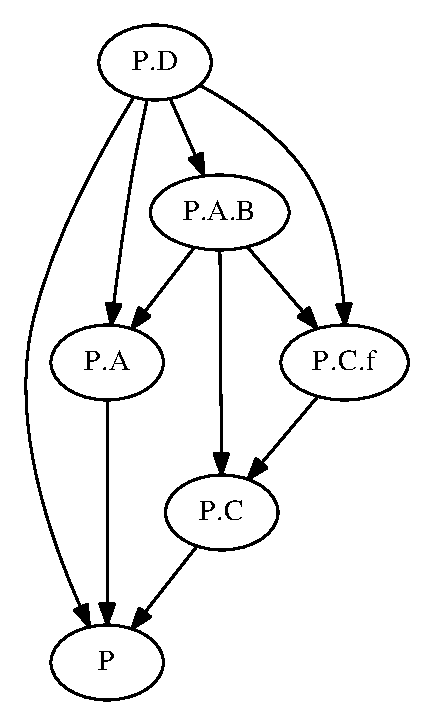
\includegraphics[]{EPS-graphs/DotAccess.eps}}}
    \qquad
    \subfloat{{\lstinputlisting[language=modelica]{modelica/DotAccess.mo}}}
    \subfloat{{\lstinputlisting[language=modelica]{modelica/DotAccessC.mo}}}
    \caption{Dot Access}
    \label{fig:dotAccess}
\end{figure}

To find the dependency from model D to function f in C, we want to add dependencies from all the parts of an Dot access. We want dependencies from D to A, A.B and C.f.
\subsection{Incremental updating}

\section{Test selection}

\chapter[Evaluation]{Evaluation}
\begin{itemize}
	\item Savings
	\item Precision
\end{itemize}

\chapter[Future Work]{Future Work}
	
\chapter[Discussion]{Discussion}


\begin{itemize}
	\item Validity
	\item Analysis granularity
\end{itemize}

\section{Related Work}
A master thesis similar to this one has previously been done at LTH. In the previously master thesis JastAdd was used to decrease the cost for testing of Android projects ~\cite{kampe2012dependroid}. There is research done on test selection. A method for safe RTS for Java has been developed before, that has many similarities with the method we are developing for Modelica. 

Studies have been conducted to investigate at which granularity dependency analysis pays off the most and how much percision it can have with out getting to expensive ~\cite{DBLP:conf/sigsoft/LegunsenHSLZM16}. It has also been done work in other techniques to achieve shorter time for testing, including dynamic test selection.

Det har tidigare gjorts ett liknande examensarbete på LTH. Där användes JastAdd för att minska kostnaden för testning av Android projekt. Det finns även forskning på området. Nästan precis samma sak som vi ska göra har gjorts tidigare men för Java ~\cite{DBLP:conf/pppj/OqvistHM16}. Utöver detta har det även tidigare undersökts hur finkornig en beroendeanalys kan vara utan att den blir för dyr ~\cite{DBLP:conf/sigsoft/LegunsenHSLZM16}. Det finns även arbete inom andra tekniker för att uppnå kortare test tider, till exempel dynamiskt testurval.

\makebibliography{thebib}

\begin{appendices}
\chapter{About This Document}
\end{appendices}


\end{document}